\documentclass[conference]{IEEEtran}
\IEEEoverridecommandlockouts
\usepackage{cite}
\usepackage{amsmath,amssymb,amsfonts}
\usepackage{graphicx}
\usepackage{textcomp}
\usepackage{xcolor}
\usepackage{url}
\usepackage[brazilian]{babel}
\usepackage[utf8]{inputenc}
\usepackage[T1]{fontenc}

\graphicspath{{../outputs/}}

\def\BibTeX{{\rm B\kern-.05em{\sc i\kern-.025em b}\kern-.08em
    T\kern-.1667em\lower.7ex\hbox{E}\kern-.125emX}}

\begin{document}

\title{Furto, Renda e Território: Uma Análise Espacial da Criminalidade\\
Patrimonial nos Municípios de São Paulo}

\author{
\IEEEauthorblockN{João Vitor Oliveira, Julio Cesar Salvino, Lucas Amorim}
\IEEEauthorblockA{Centro de Matemática, Computação e Cognição\\
Universidade Federal do ABC (UFABC)\\
Orientação: Prof.\textsuperscript{a} Flávia da Fonseca Feitosa\\
Análise de Dados para Planejamento Territorial}
}

\maketitle

\begin{abstract}
Este trabalho investiga se municípios mais pobres do estado de São Paulo
apresentam maiores taxas de criminalidade patrimonial, cruzando ocorrências
registradas pela SSP-SP (2025) com a renda média per capita do Censo IBGE 2022
nos 645 municípios do estado. Partindo de uma análise exploratória e de
correlação, mostramos que a relação entre renda e taxa de furto é, ao
contrário da hipótese inicial, positiva. Investigamos essa relação com um
ferramental progressivo de econometria espacial --- correlação,
autocorrelação espacial global e local (Moran's I e LISA), regressão linear
clássica, regressão espacial global (\textit{spatial lag} e \textit{spatial
error}) e regressão geograficamente ponderada (GWR) --- incorporando uma
variável de condição litorânea/turística. O modelo final (GWR com renda e
litoral) eleva o poder explicativo de $R^2=0{,}129$ (OLS simples) para
$R^2=0{,}532$, com o menor AIC entre os modelos testados. Os resultados
indicam que a criminalidade patrimonial responde muito mais à condição
litorânea/turística e à não-estacionariedade espacial da relação
renda--furto do que à renda em si, isoladamente.
\end{abstract}

\begin{IEEEkeywords}
análise espacial, autocorrelação espacial, regressão geograficamente
ponderada, criminalidade, planejamento territorial
\end{IEEEkeywords}

\section{Introdução}

A pergunta que orienta este trabalho é direta: acontecem mais crimes nas
cidades mais pobres? Essa hipótese (H1), amplamente difundida no senso comum
sobre criminalidade, foi o ponto de partida da pesquisa, desenvolvida na
disciplina de Análise de Dados para Planejamento Territorial da UFABC. Para
testá-la, tomamos como variável dependente a taxa de furto (art. 155) por
1.000 habitantes dos 645 municípios de São Paulo e como variável explicativa
a renda média per capita.

Optamos por trabalhar com taxas, e não contagens brutas de ocorrências,
porque a contagem acompanha o tamanho da população: qualquer mapa de
contagem destaca a capital e as cidades grandes independentemente do
fenômeno investigado, enquanto a taxa permite comparar municípios de portes
muito diferentes.

Ao longo da análise exploratória, emergiu uma segunda hipótese (H2):
municípios litorâneos e turísticos concentram taxas de criminalidade
patrimonial mais altas, não porque sejam mais pobres, mas porque sua
população flutuante de verão infla o numerador da taxa (ocorrências) sobre
um denominador que mede apenas a população residente. Essa hipótese
exploratória guiou boa parte do desenvolvimento metodológico deste trabalho,
da regressão múltipla à regressão geograficamente ponderada (GWR).

O restante deste artigo está organizado da seguinte forma: a Seção II
descreve os dados e variáveis utilizados; a Seção III apresenta a
metodologia; a Seção IV percorre o desenvolvimento da análise, do
exploratório à GWR; e a Seção V conclui.

\section{Dados e Variáveis}

A unidade de análise são os 645 municípios do estado de São Paulo, com dados
de criminalidade da SSP-SP \cite{sspsp} e de renda e população do Censo IBGE
2022 \cite{ibge}. A Tabela \ref{tab:variaveis} resume as variáveis
utilizadas.

\begin{table}[htbp]
\caption{Variáveis utilizadas na análise}
\label{tab:variaveis}
\centering
\begin{tabular}{p{1.7cm}p{1.6cm}p{4.3cm}}
\hline
\textbf{Variável} & \textbf{Fonte} & \textbf{Descrição} \\
\hline
Taxa de roubo (art. 157) & SSP-SP, 2025 & Ocorrências por 1.000 hab. \\
Taxa de furto (art. 155) & SSP-SP, 2025 & Ocorrências por 1.000 hab. \\
Taxa de lesão corporal (art. 129) & SSP-SP, 2025 & Ocorrências por 1.000 hab. \\
Renda média & IBGE, Censo 2022 & Renda per capita em R\$ \\
População & IBGE, Tabela 4709 & Denominador das taxas \\
Litorâneo/turístico & Classificação do grupo & Dummy (1/0), 16 municípios da costa paulista \\
\hline
\end{tabular}
\end{table}

A junção entre as bases criminal e de renda usa o código IBGE de 7 dígitos
como chave, nunca o nome do município: a base da SSP abrevia nomes (ex.
``S BARBARA D OESTE''), o que exige uma resolução em cascata (correspondência
exata $\rightarrow$ expansão de abreviações $\rightarrow$ remoção de
preposições $\rightarrow$ distância de edição $\leq 1$) para evitar perdas de
observações.

Entre os três crimes disponíveis, o furto foi escolhido como variável
dependente principal por apresentar a relação mais nítida com renda e
território ao longo da análise exploratória.

\section{Metodologia}

A vizinhança espacial utilizada em todas as etapas é a contiguidade
\textit{queen} de ordem 1 (dois municípios são vizinhos se compartilham
qualquer trecho de fronteira), com pesos normalizados por linha
(\textit{row-standardization}). Essa matriz tem 645 observações, mínimo de 0
e máximo de 22 vizinhos, média de 5,50. Ilhabela, por ser arquipélago, fica
sem vizinhos (\texttt{zero.policy = TRUE}).

A análise segue quatro etapas progressivas:

\begin{enumerate}
\item \textbf{Correlação e autocorrelação espacial:} correlações de Pearson
e Spearman entre as taxas de crime e a renda; índice global de Moran
\cite{moran1950} e sua decomposição local (LISA) \cite{anselin1995}, com
significância avaliada por permutação condicional (999 permutações), mais
robusta que a versão analítica para variáveis assimétricas com muitos zeros.
\item \textbf{Regressão linear clássica (OLS):} modelo simples
(taxa $\sim$ renda) e múltiplo (taxa $\sim$ renda + litoral), com diagnóstico
de resíduos (Shapiro-Wilk, \texttt{ncvTest}, distância de Cook).
\item \textbf{Regressão espacial global:} testes de Multiplicadores de
Lagrange (LM) para escolher entre \textit{spatial lag} ($\rho$) e
\textit{spatial error} ($\lambda$), ambos por máxima verossimilhança.
\item \textbf{Regressão Geograficamente Ponderada (GWR)} \cite{fotheringham2002}:
ajusta uma regressão local para cada município, com pesos decaindo por um
núcleo gaussiano $w_{ij} = \exp\left(-\frac{1}{2}(d_{ij}/h)^2\right)$ em
função da distância geográfica $d_{ij}$, onde a banda $h$ é adaptativa
(definida pelo $k$-ésimo vizinho mais próximo, $k \approx 10$, escolhido por
validação cruzada).
\end{enumerate}

\section{Desenvolvimento e Resultados}

\subsection{Análise exploratória}

A Fig. \ref{fig:mapa_furto} mostra a distribuição espacial da taxa de furto
por 1.000 habitantes. O padrão visual já sugere concentração na
macrometrópole e no litoral, contrariando a intuição de que a criminalidade
patrimonial se concentraria nas regiões mais pobres do interior.

\begin{figure}[htbp]
\centering
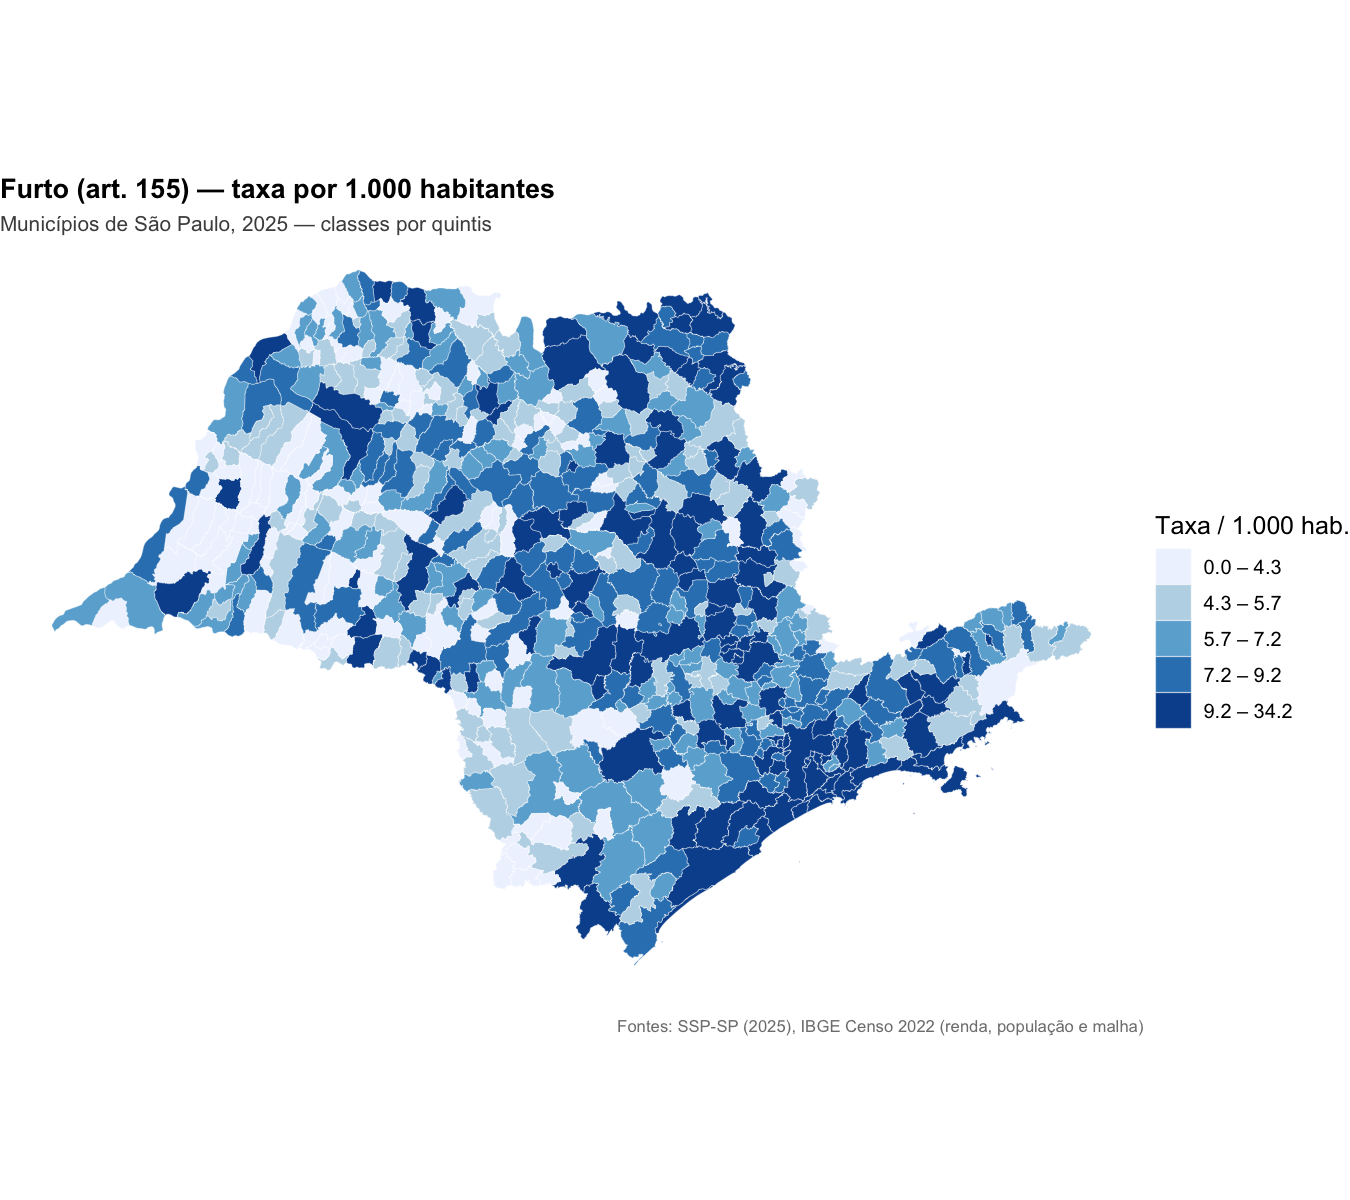
\includegraphics[width=0.9\linewidth]{mapa_taxa_furto.png}
\caption{Taxa de furto por 1.000 habitantes, municípios de SP (classes por
quintis).}
\label{fig:mapa_furto}
\end{figure}

Mapas complementares (por desvio padrão e \textit{box map}, não reproduzidos
aqui por espaço) confirmam o padrão: o \textit{box map} identifica 17
outliers superiores na taxa de furto, concentrados no litoral e na capital,
contra 60 outliers superiores na taxa de roubo, quase todos contíguos na
RMSP e na Baixada Santista.

A dispersão de cada taxa contra a renda média (Fig. \ref{fig:dispersoes})
ajuda a justificar a escolha do furto como variável dependente principal:
no roubo, o outlier mais extremo é de um município não litorâneo, e os
litorâneos aparecem elevados sem dominar o topo da distribuição; na lesão
corporal, o outlier extremo é de renda baixíssima e não litorâneo, com os
litorâneos perdidos no meio da nuvem de pontos; já no furto, os outliers
extremos são quase todos litorâneos --- Mongaguá e outros municípios da
costa aparecem bem acima da nuvem geral. É o único dos três crimes em que o
padrão litorâneo aparece nitidamente nos extremos da distribuição.

\begin{figure}[htbp]
\centering
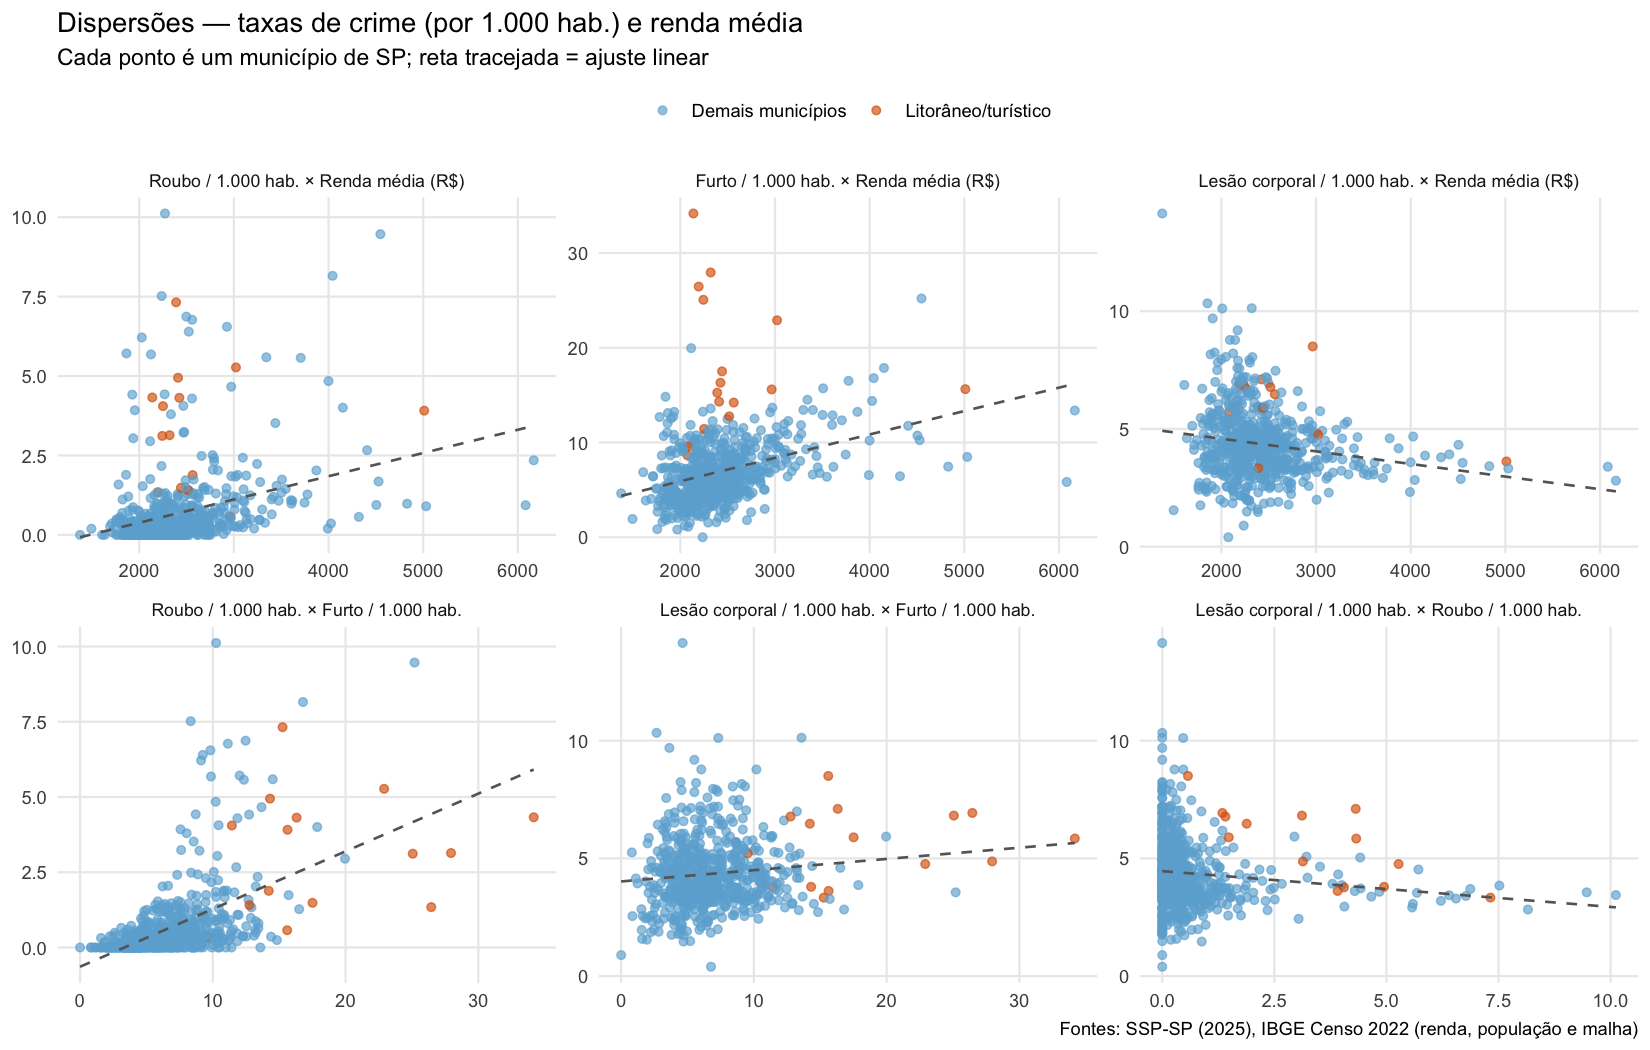
\includegraphics[width=0.9\linewidth]{dispersoes_taxas_renda.png}
\caption{Dispersão das taxas de roubo, furto e lesão corporal (por 1.000
hab.) contra a renda média, com destaque para os municípios
litorâneos/turísticos.}
\label{fig:dispersoes}
\end{figure}

\subsection{Correlação}

A Tabela \ref{tab:correlacao} mostra as correlações entre as taxas de crime
e a renda média. Roubo e furto correlacionam \textit{positivamente} com a
renda --- o oposto do que H1 previa --- enquanto a lesão corporal
correlaciona negativamente, embora de forma fraca.

\begin{table}[htbp]
\caption{Correlação entre taxas de crime e renda}
\label{tab:correlacao}
\centering
\begin{tabular}{lcc}
\hline
\textbf{Par} & \textbf{Pearson} & \textbf{Spearman} \\
\hline
Roubo $\times$ Renda & 0,302 & 0,389 \\
Furto $\times$ Renda & 0,359 & 0,380 \\
Lesão corporal $\times$ Renda & $-$0,190 & $-$0,166 \\
\hline
\end{tabular}
\end{table}

\begin{figure}[htbp]
\centering
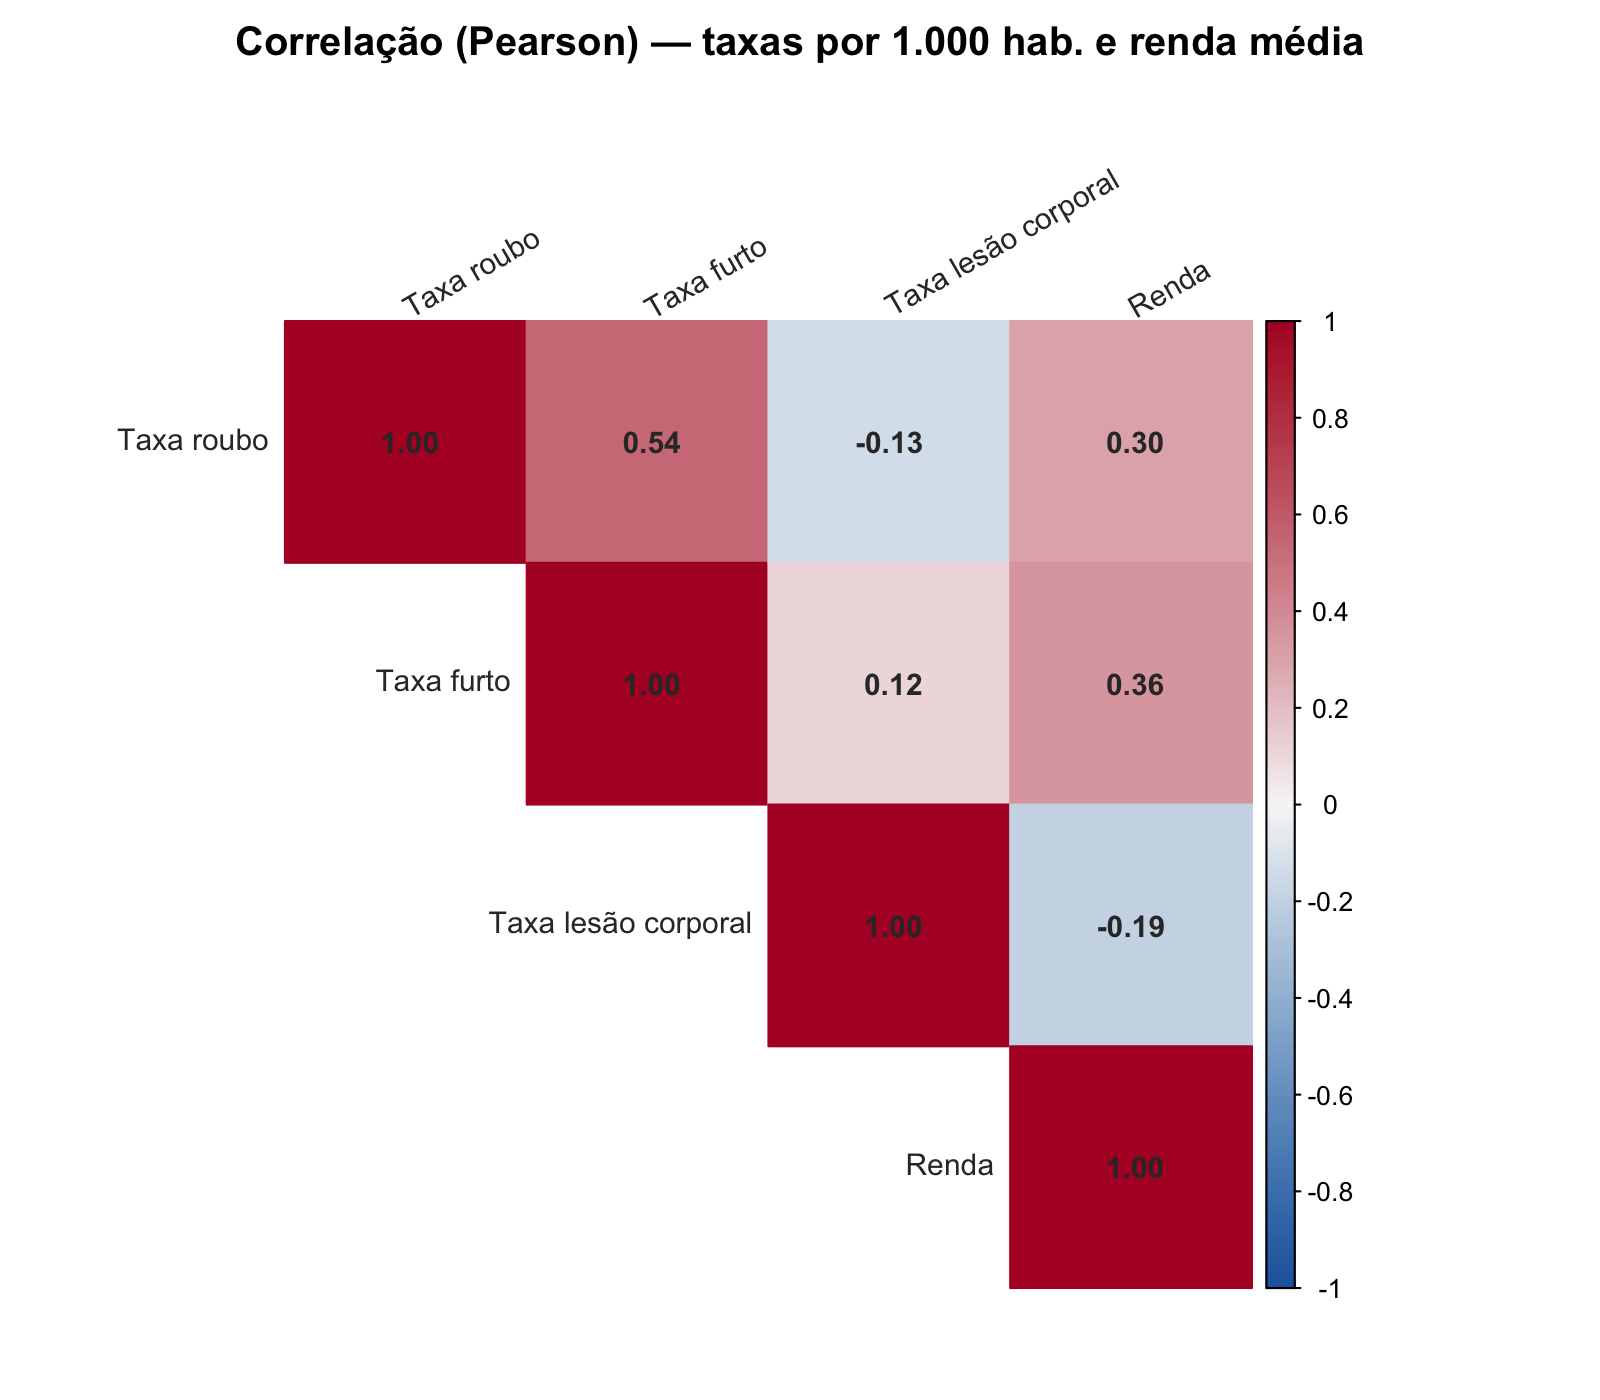
\includegraphics[width=0.9\linewidth]{correlacao_matriz.png}
\caption{Matriz de correlação entre as taxas de crime e a renda média.}
\label{fig:correlacao}
\end{figure}

\subsection{Autocorrelação espacial: Moran global e LISA}

O índice global de Moran \cite{moran1950} mede o grau em que valores
semelhantes se aglomeram no espaço, operacionalizando a chamada primeira lei
da geografia --- a ideia de que lugares próximos tendem a se parecer mais
entre si do que lugares distantes \cite{tobler1970}. A Tabela
\ref{tab:moran} mostra que a taxa de roubo tem autocorrelação espacial forte
($I=0{,}832$), a de furto moderada ($I=0{,}422$) e a de lesão corporal fraca
($I=0{,}181$), todas significativas a $p=0{,}001$ por permutação (999
simulações).

\begin{table}[htbp]
\caption{Índice global de Moran por crime}
\label{tab:moran}
\centering
\begin{tabular}{lccc}
\hline
\textbf{Variável} & \textbf{Moran's I} & \textbf{p (perm.)} & \textbf{Leitura} \\
\hline
Taxa de roubo & 0,832 & 0,001 & forte \\
Taxa de furto & 0,422 & 0,001 & moderada \\
Taxa de lesão corporal & 0,181 & 0,001 & fraca \\
\hline
\end{tabular}
\end{table}

A decomposição local (LISA \cite{anselin1995}, Fig. \ref{fig:lisa}) mostra,
para o furto, 36 municípios no cluster Alto-Alto acompanhando o litoral de
Ubatuba a Cananéia, e 45 municípios Baixo-Baixo no oeste e centro-sul. Dos
municípios do cluster Alto-Alto, 36\% são litorâneos ou turísticos ---
primeira evidência quantitativa a favor de H2.\footnote{Os mesmos dados
processados no GeoDa (permutação condicional independente) indicam 49
municípios Alto-Alto e 67 Baixo-Baixo para o furto --- a mesma geografia de
clusters, com contagens um pouco maiores. Reportamos aqui os números do R
(\texttt{spdep::localmoran\_perm}), a mesma implementação usada no Moran's I
global da Tabela \ref{tab:moran}, para manter os dois números
consistentes entre si; ver \texttt{docs/guia\_geoda.md} para a comparação
completa R $\times$ GeoDa.}

\begin{figure}[htbp]
\centering
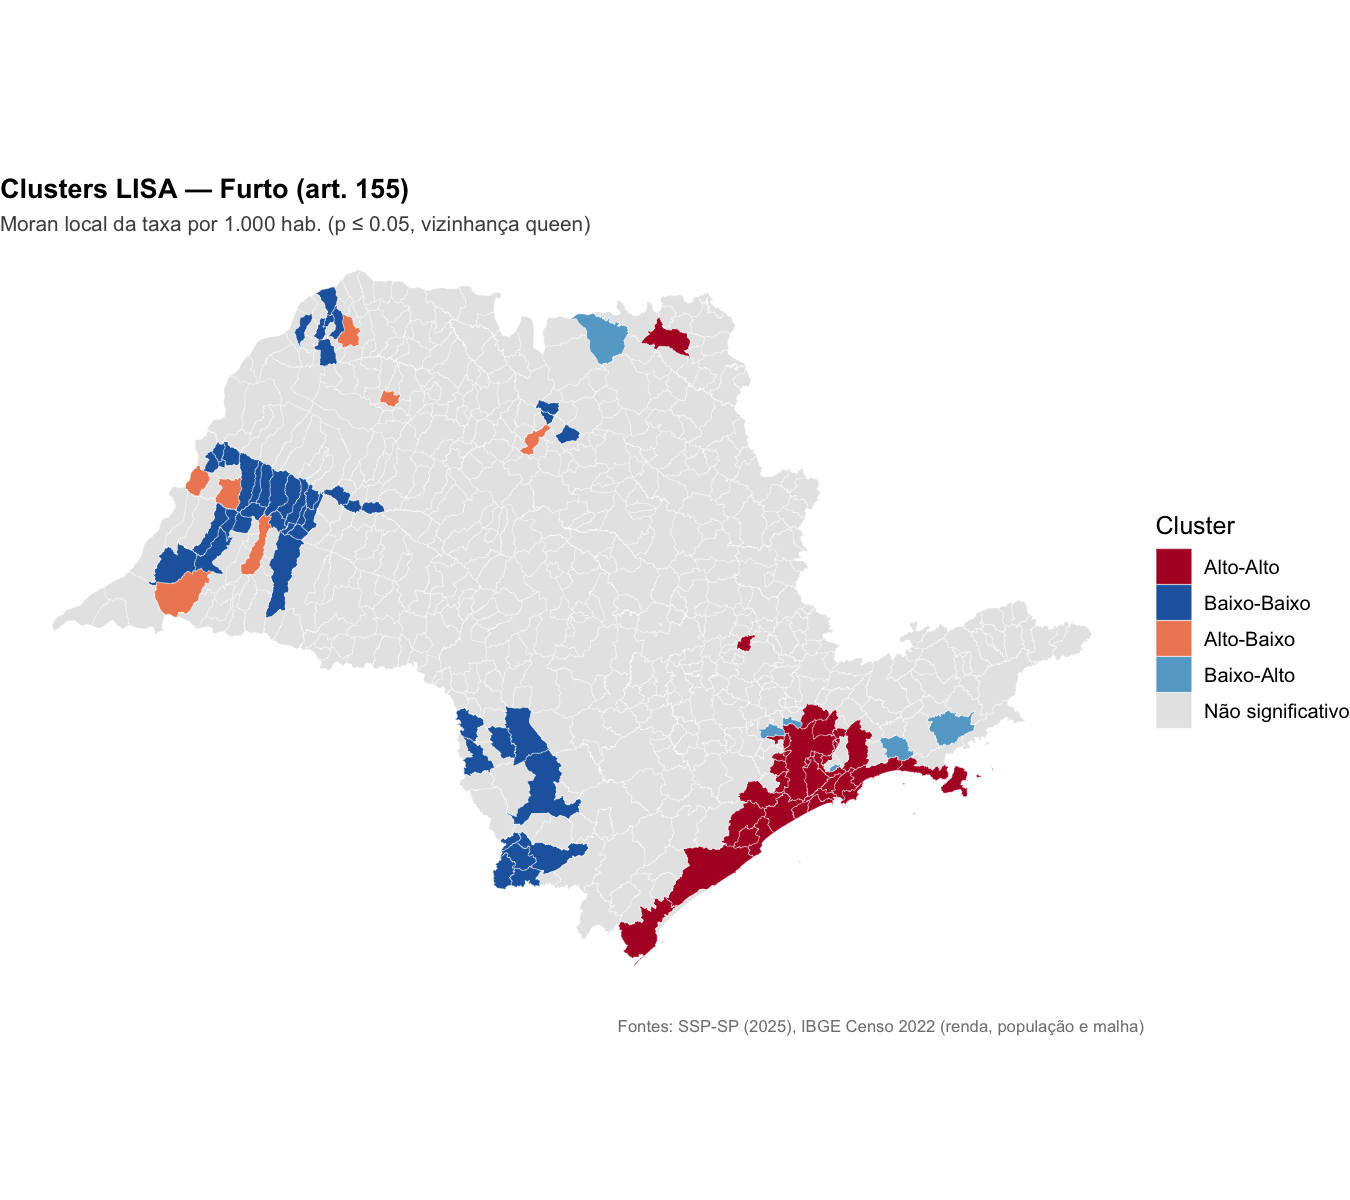
\includegraphics[width=0.9\linewidth]{mapa_lisa_furto.png}
\caption{Clusters LISA da taxa de furto ($p \leq 0{,}05$, vizinhança queen).}
\label{fig:lisa}
\end{figure}

\subsection{Regressão linear clássica}

O modelo simples (Fig. \ref{fig:reg_simples}) estima:
\begin{equation}
\text{taxa de furto} = 0{,}971 + 0{,}00247 \cdot \text{renda}, \quad R^2 = 0{,}129
\label{eq:ols_simples}
\end{equation}
O coeficiente positivo e significativo ($p<0{,}001$) confirma que a
hipótese H1 não se sustenta: mais renda está associada a \textit{mais}
furto, não menos. O $R^2$ de 0,129 indica, porém, baixo poder explicativo
isolado.

\begin{figure}[htbp]
\centering
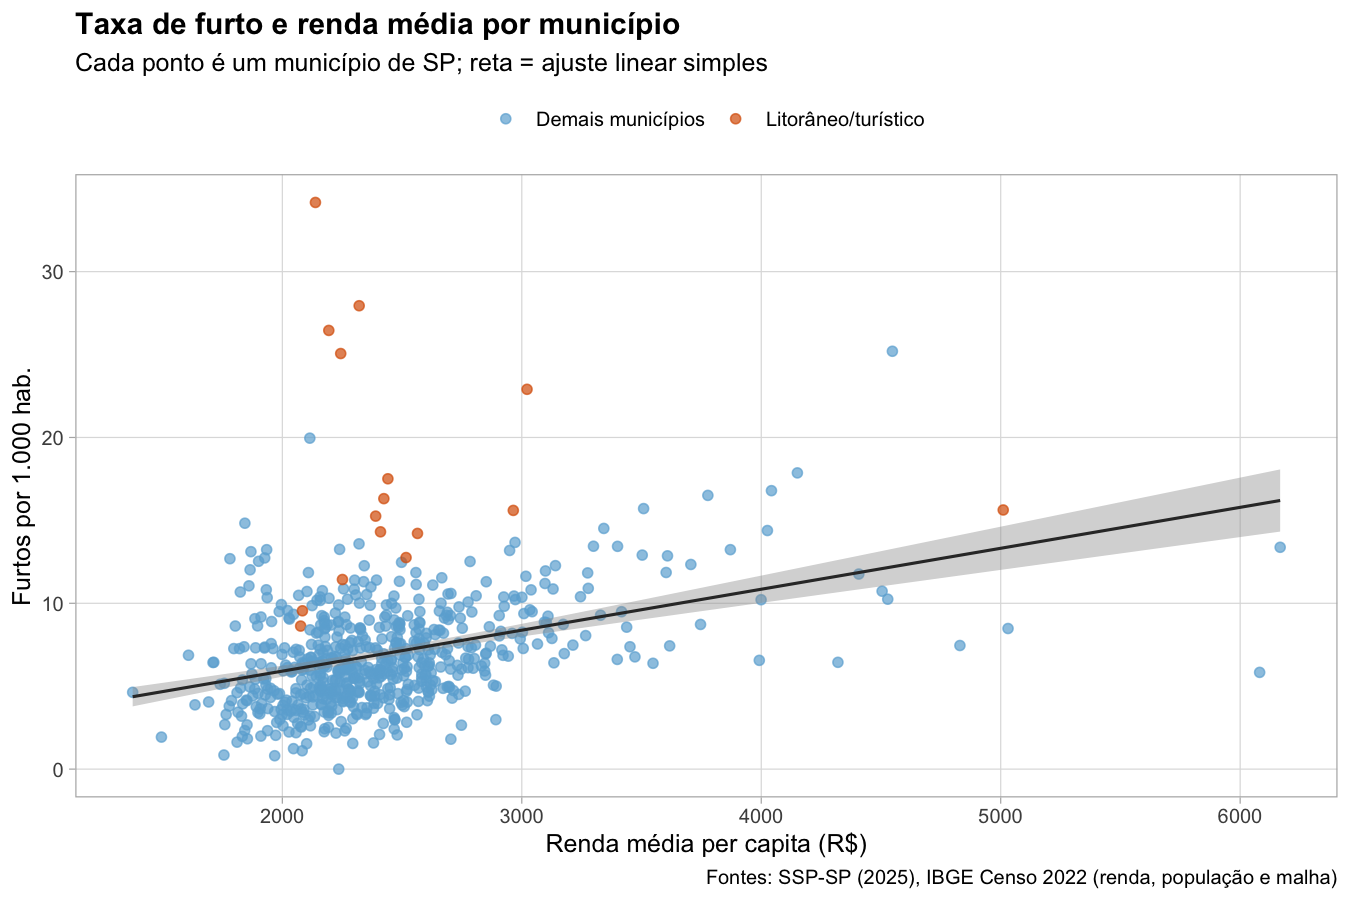
\includegraphics[width=0.9\linewidth]{reg_dispersao.png}
\caption{Taxa de furto contra renda média, com reta de tendência.}
\label{fig:reg_simples}
\end{figure}

A distância de Cook identifica 29 municípios influentes (Fig.
\ref{fig:cook}); ao excluí-los, a inclinação da renda sobe de 0,00247 para
0,00288 e o $R^2$ de 0,13 para 0,19 --- ou seja, o efeito positivo não é
artefato de poucos pontos extremos, e se fortalece sem eles. Os municípios
mais influentes são, no entanto, informativos: Mongaguá e outros litorâneos
ficam muito acima da reta, e Santana de Parnaíba (renda alta, furto baixo)
puxa a reta para baixo pela direita.

\begin{figure}[htbp]
\centering
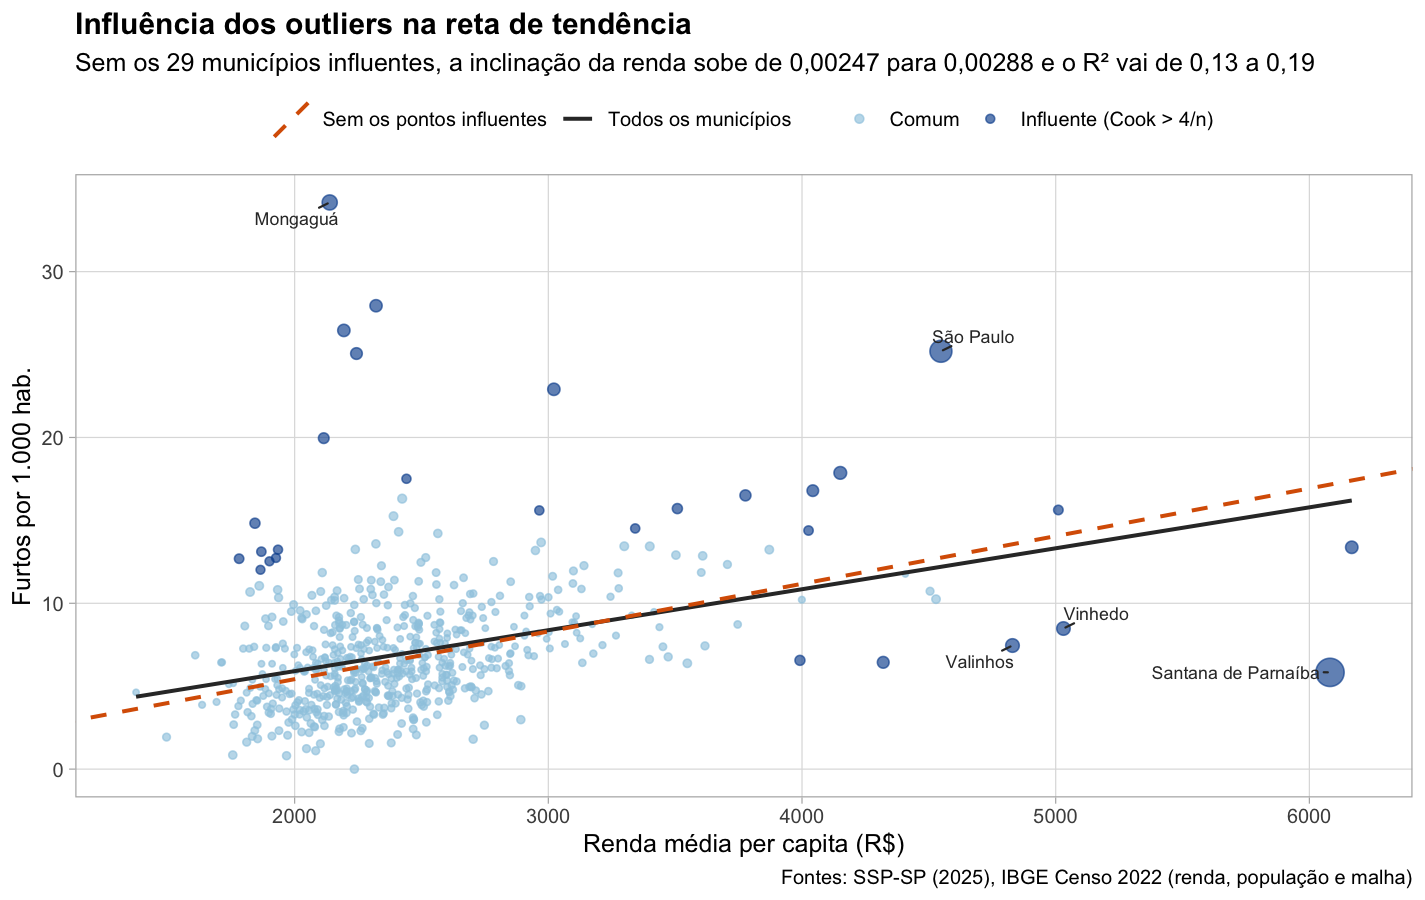
\includegraphics[width=0.9\linewidth]{reg_outliers.png}
\caption{Influência dos municípios na reta de tendência (distância de
Cook).}
\label{fig:cook}
\end{figure}

Isso motiva incluir explicitamente a condição litorânea/turística como
variável dummy:
\begin{equation}
\text{taxa de furto} = 1{,}036 + 0{,}00233 \cdot \text{renda} + 10{,}969 \cdot \text{litoral}
\label{eq:ols_multiplo}
\end{equation}
com $R^2 = 0{,}357$ ($R^2_{\text{ajustado}} = 0{,}355$). O coeficiente da
renda pouco muda em relação ao modelo simples (VIF=1, sem
multicolinearidade), e o termo litoral, de 10,969, é a distância vertical
entre as retas dos dois grupos (Fig. \ref{fig:reg_multipla}): um município
litorâneo registra, em média, quase 11 furtos a mais por 1.000 habitantes
do que um município comum de mesma renda --- efeito equivalente a uma
diferença de renda de cerca de R\$4.700.

\begin{figure}[htbp]
\centering
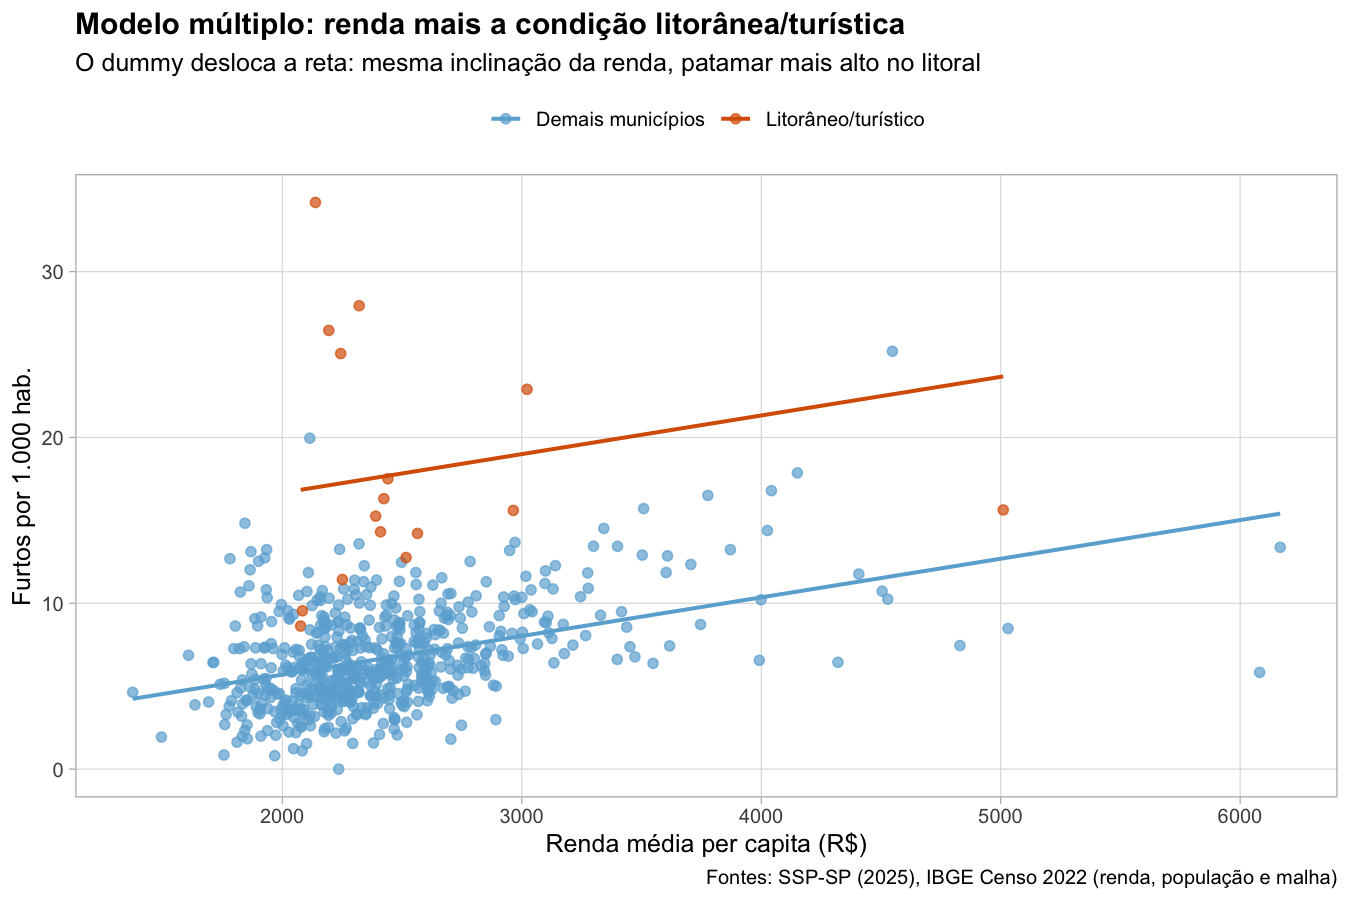
\includegraphics[width=0.9\linewidth]{reg_multipla.png}
\caption{Modelo múltiplo: retas paralelas por condição litorânea.}
\label{fig:reg_multipla}
\end{figure}

Diagnósticos formais (Shapiro-Wilk, \texttt{ncvTest}, ambos $p<0{,}001$)
rejeitam normalidade e homocedasticidade dos resíduos --- esperado dada a
assimetria das taxas de crime --- e motivam avançar para modelos que tratem
a estrutura espacial dos dados.

\subsection{Regressão espacial global}

O Moran's I dos resíduos do modelo clássico é 0,38 ($p<0{,}001$): a
autocorrelação espacial não explicada é elevada, violando a premissa de
independência do OLS. Os testes de Multiplicadores de Lagrange (Tabela
\ref{tab:lm}) indicam, pela versão robusta, o modelo \textit{spatial error}
como mais adequado (Robust LM error significativo, Robust LM lag não
significativo).

\begin{table}[htbp]
\caption{Testes de Multiplicadores de Lagrange}
\label{tab:lm}
\centering
\begin{tabular}{lcc}
\hline
\textbf{Teste} & \textbf{Estatística} & \textbf{p-valor} \\
\hline
LM (lag) & 217,4 & $<0{,}001$ \\
LM (error) & 238,9 & $<0{,}001$ \\
Robust LM (lag) & 1,23 & 0,267 \\
Robust LM (error) & 22,8 & $<0{,}001$ \\
\hline
\end{tabular}
\end{table}

O modelo \textit{spatial error} ($\lambda = 0{,}588$, $R^2 = 0{,}392$,
AIC$=3220{,}6$) supõe que a dependência espacial está no erro, refletindo
uma variável omitida e espacialmente agrupada --- coerente com a hipótese de
que é a condição litorânea, e não um efeito de contágio entre vizinhos, que
gera o padrão espacial. Após o ajuste, o Moran's I dos resíduos cai de 0,38
para $-0{,}03$, praticamente eliminando a autocorrelação residual.

\subsection{Regressão Geograficamente Ponderada (GWR)}

O GWR relaxa a suposição de que a relação renda--furto é constante no
espaço. Com banda adaptativa ($k \approx 10$ vizinhos), o $R^2$
quase-global sobe para 0,458 (Fig. \ref{fig:gwr_r2}), superando os modelos
globais. O coeficiente local da renda varia de $-0{,}00216$ a $+0{,}00562$
pelo estado, positivo na maior parte e invertido num bolsão do noroeste; a
estatística $t$ é significativa ($|t| > 1{,}96$) em 72\% dos municípios.

\begin{figure}[htbp]
\centering
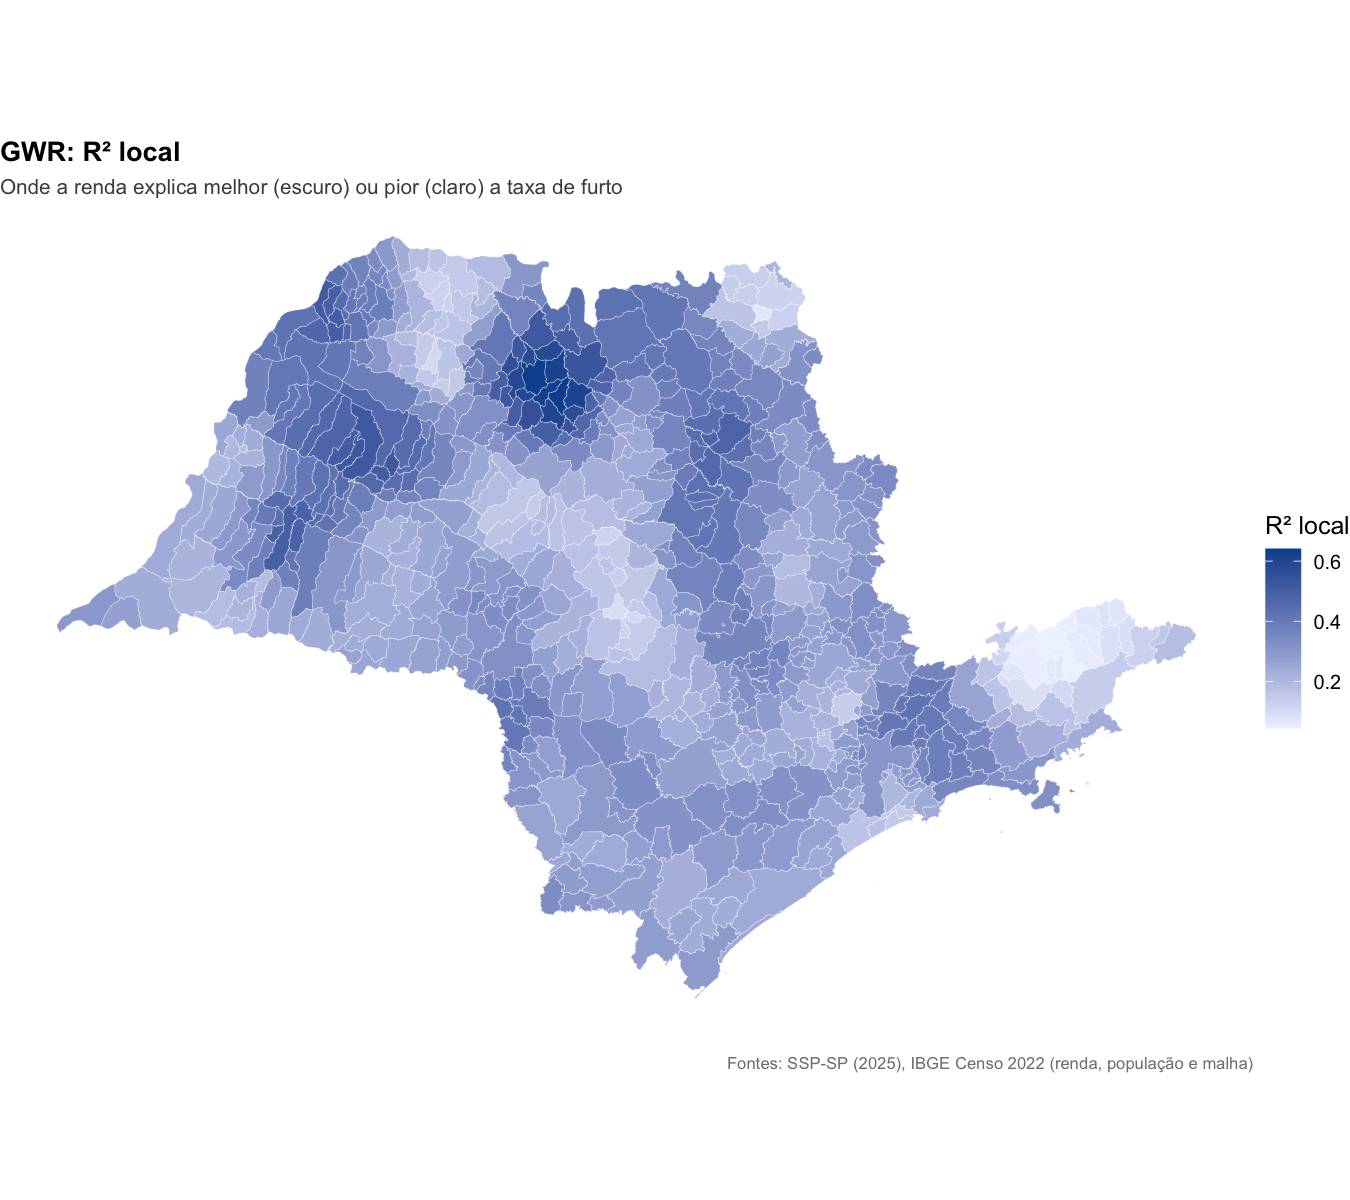
\includegraphics[width=0.9\linewidth]{reg_esp_gwr_r2.png}
\caption{$R^2$ local do GWR (taxa de furto $\sim$ renda).}
\label{fig:gwr_r2}
\end{figure}

O $R^2$ local varia de 0,05 a 0,64: a renda explica bem a taxa de furto no
centro-oeste do estado e mal no litoral e na Região Metropolitana ---
justamente onde a população flutuante turística deveria dominar o
fenômeno, segundo H2.

\subsection{GWR com a variável litorânea e cenário contrafactual}

Ajustando GWR com renda \textit{e} litoral, o $R^2$ quase-global sobe para
0,532 e o AIC cai para 3027,4, o melhor entre todos os modelos testados
(Tabela \ref{tab:comparacao}). Os coeficientes locais (Fig.
\ref{fig:gwr_coef}) mostram que o efeito litorâneo varia de 0 a 22
furtos/1.000 hab. conforme o município.

\begin{figure}[htbp]
\centering
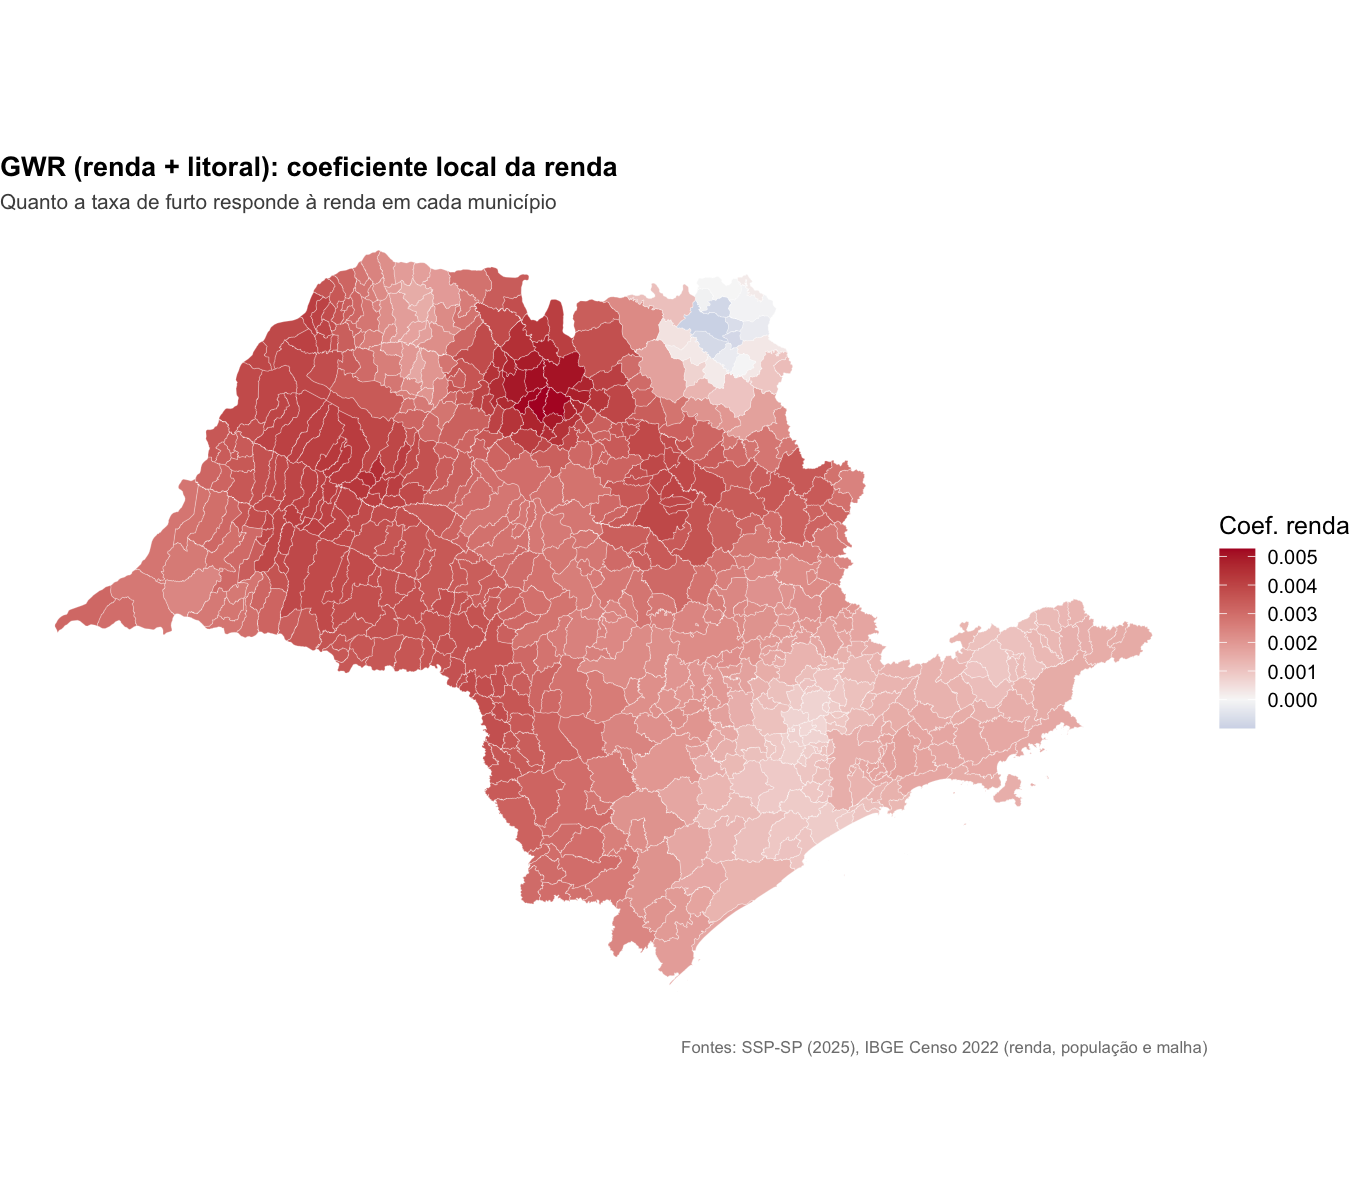
\includegraphics[width=0.48\linewidth]{gwr_lit_coef_renda.png}
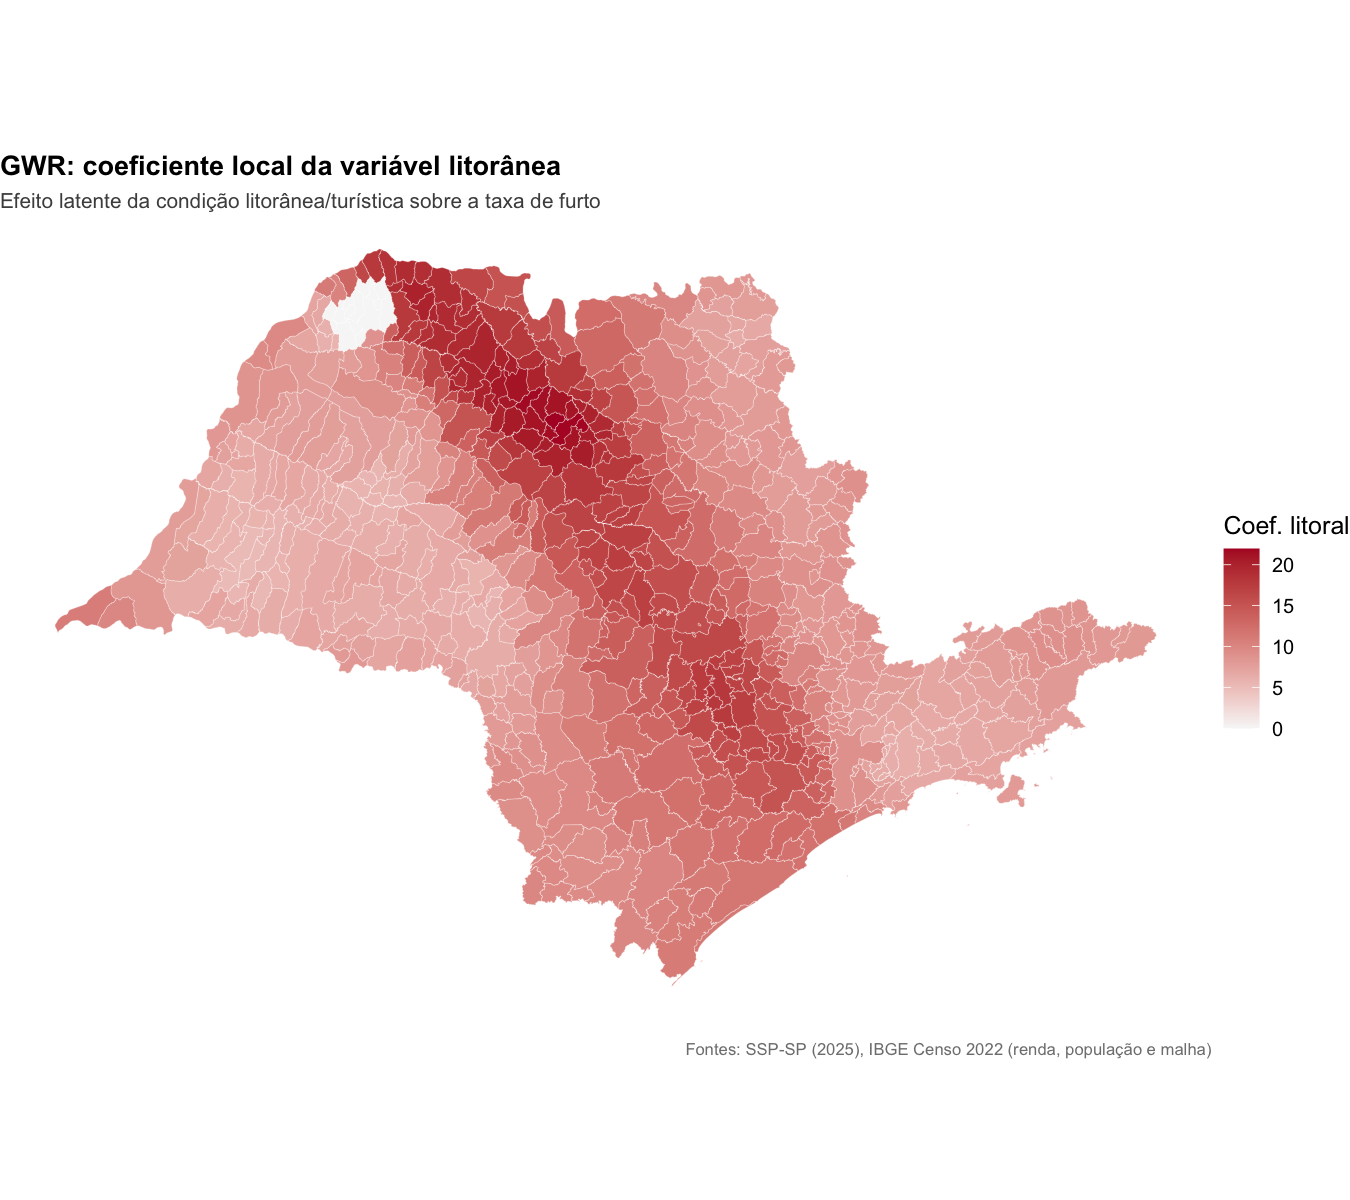
\includegraphics[width=0.48\linewidth]{gwr_lit_coef_litoral.png}
\caption{Coeficientes locais da renda (esq.) e da condição litorânea (dir.),
modelo GWR com as duas variáveis.}
\label{fig:gwr_coef}
\end{figure}

Complementarmente, a Fig. \ref{fig:gwr_t} mapeia a estatística $t$ local de
cada variável --- uma leitura contínua de magnitude e significância, mais
informativa que um simples corte binário em $|t| > 1{,}96$: o efeito da
renda é significativo (|t|>1,96) na quase totalidade do estado, com exceção
de um bolsão no extremo noroeste; o efeito litorâneo é significativo em
praticamente todos os municípios, mas sua magnitude cresce à medida que se
caminha do noroeste em direção à metade sul-sudeste do estado, com o pico
concentrado na faixa que vai da Região Metropolitana à Baixada Santista ---
coerente com a leitura de que o efeito litorâneo se espalha por contágio
espacial do GWR para além dos 16 municípios classificados como
litorâneos/turísticos, e não fica restrito a uma faixa estreita no litoral.

\begin{figure}[htbp]
\centering
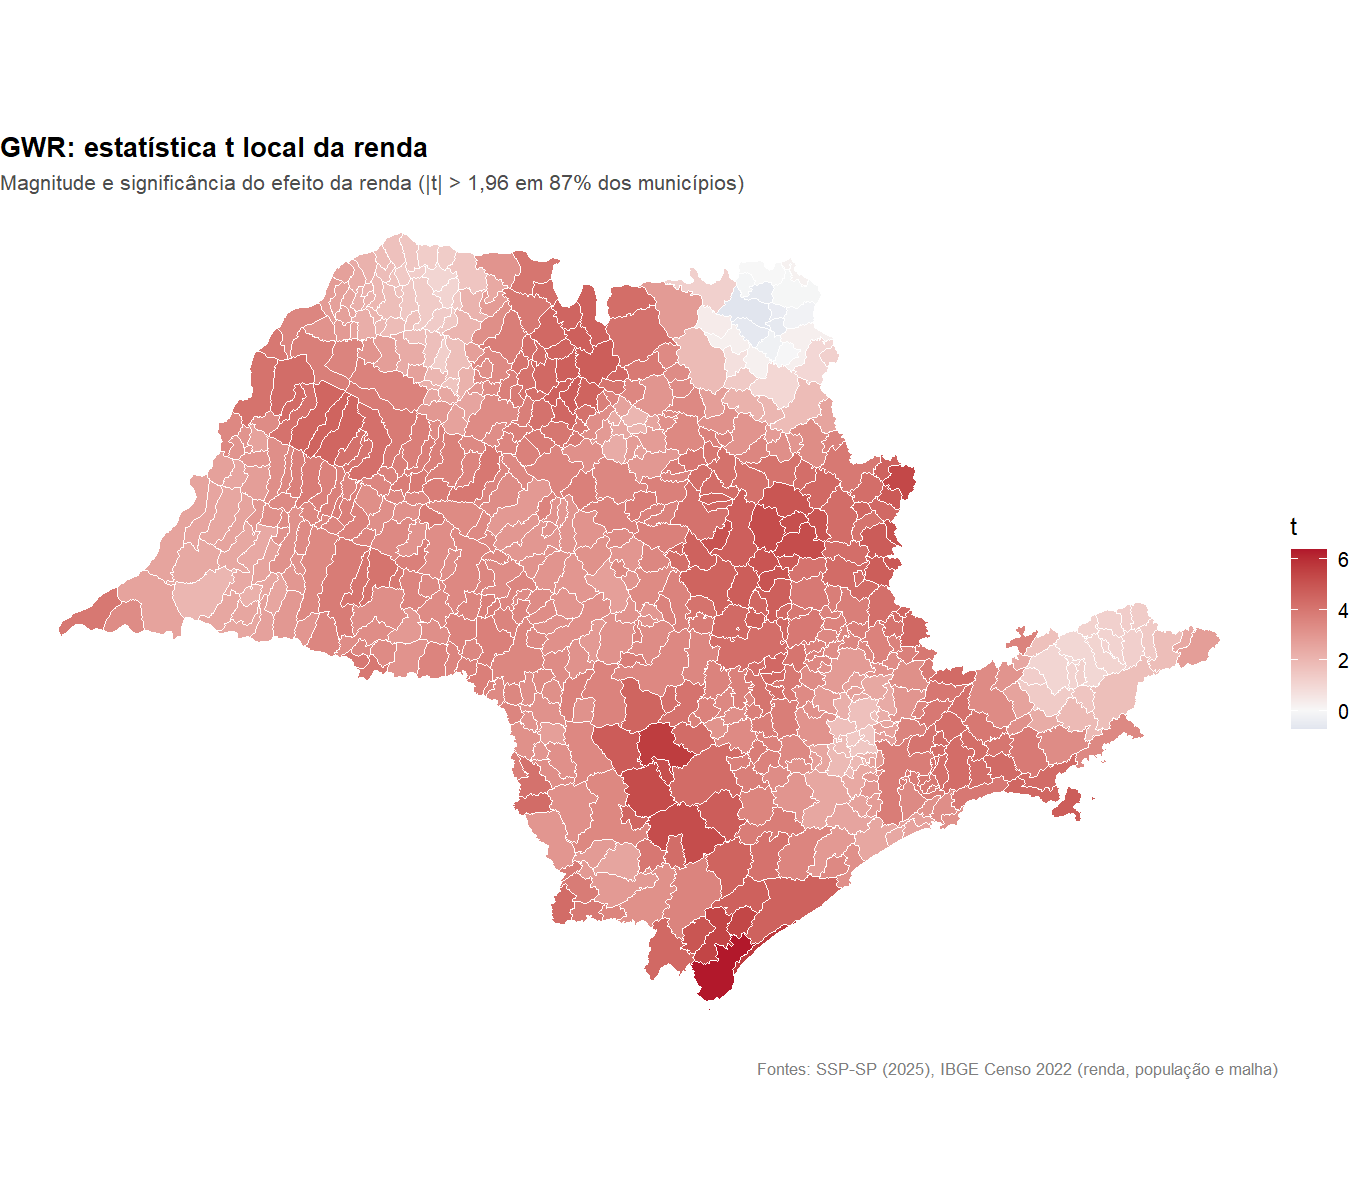
\includegraphics[width=0.48\linewidth]{gwr_lit_t_renda.png}
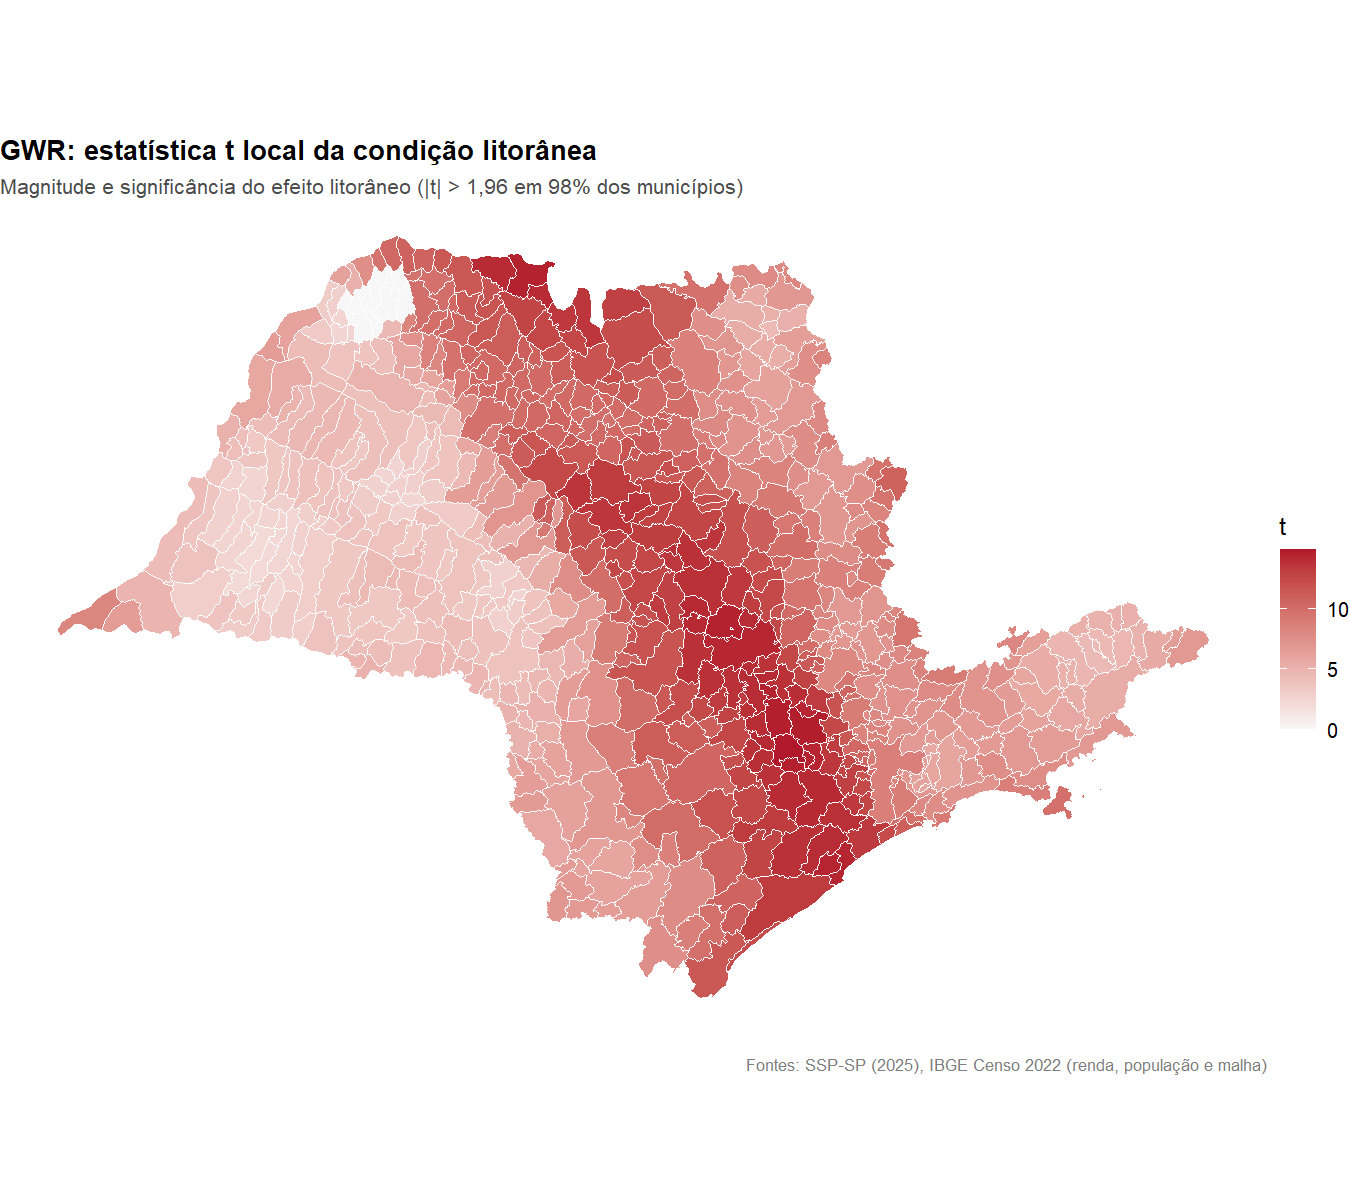
\includegraphics[width=0.48\linewidth]{gwr_lit_t_litoral.png}
\caption{Estatística $t$ local da renda (esq.) e da condição litorânea
(dir.), modelo GWR com as duas variáveis.}
\label{fig:gwr_t}
\end{figure}

Para isolar o efeito litorâneo, construímos um cenário contrafactual:
mantendo os coeficientes locais do GWR, zeramos a variável litoral e
recalculamos a predição (Fig. \ref{fig:contrafactual}). A diferença entre a
predição real e a contrafactual --- de até 12 furtos/1.000 hab. ---
concentra-se inteiramente na faixa costeira.

\begin{figure}[htbp]
\centering
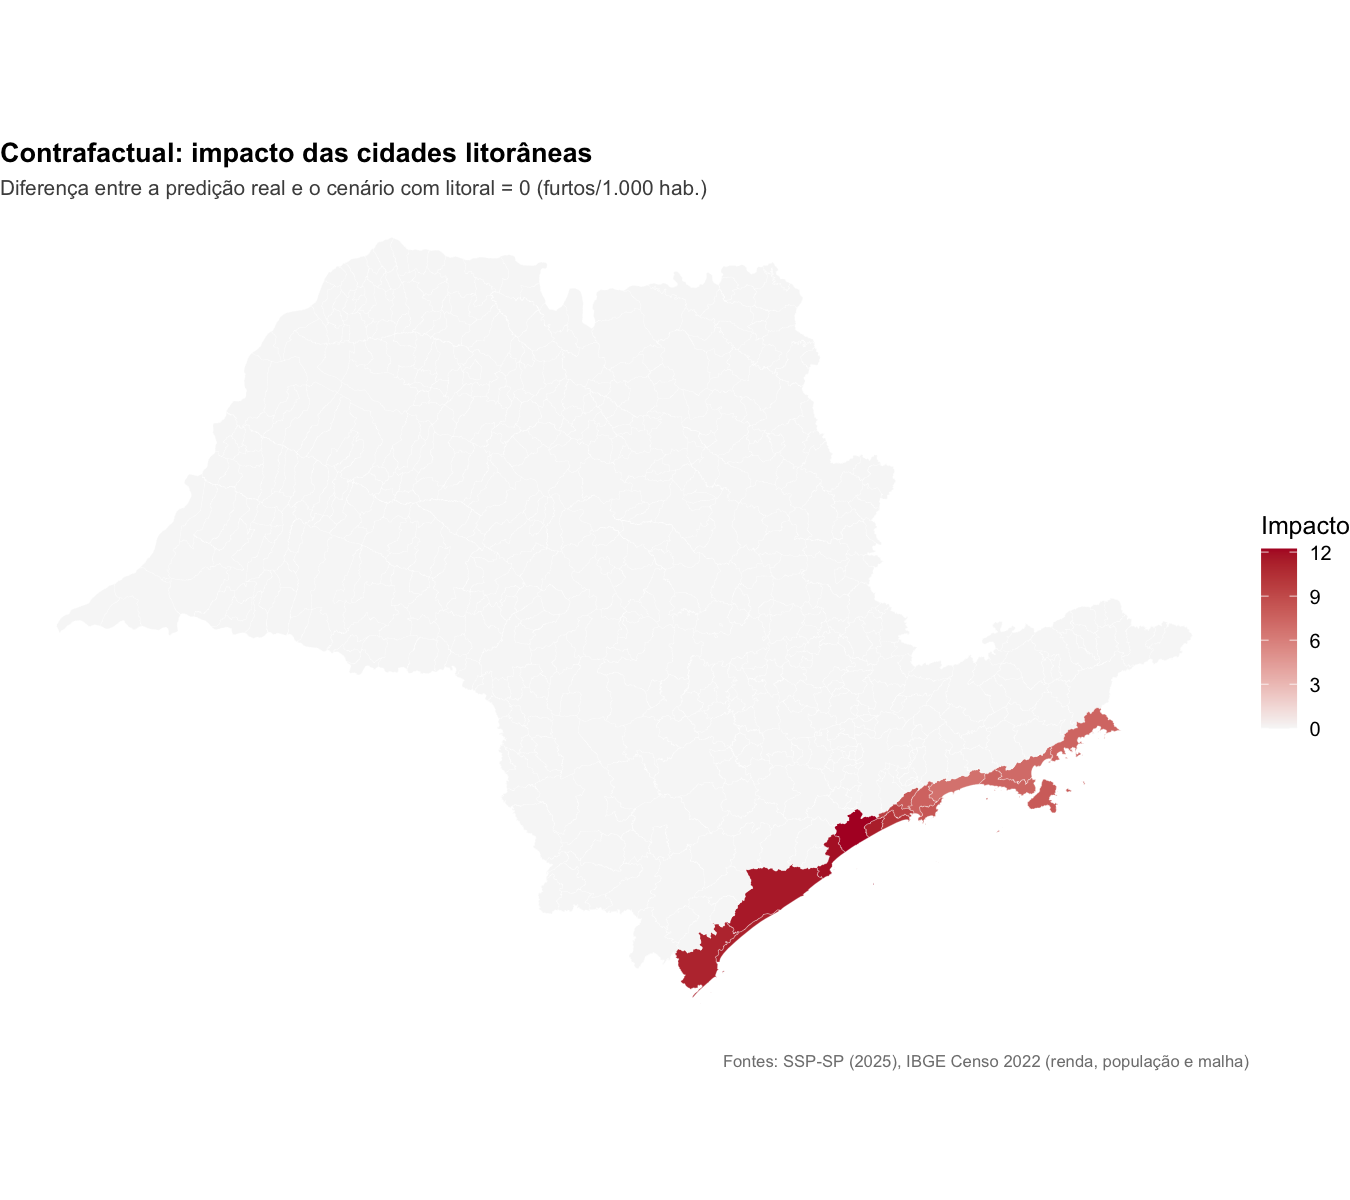
\includegraphics[width=0.9\linewidth]{gwr_contrafactual_dif.png}
\caption{Impacto contrafactual da condição litorânea sobre a taxa de furto
prevista.}
\label{fig:contrafactual}
\end{figure}

Como leitura complementar, ajustamos regressões separadas por regime
espacial (Fig. \ref{fig:regime}): no interior, a taxa de furto cresce com a
renda ($R^2 = 0{,}19$); no litoral, a reta é praticamente plana, num
patamar bem mais alto ($R^2 = 0{,}008$) --- ou seja, dentro do próprio
grupo litorâneo, a renda não explica a variação do furto.

\begin{figure}[htbp]
\centering
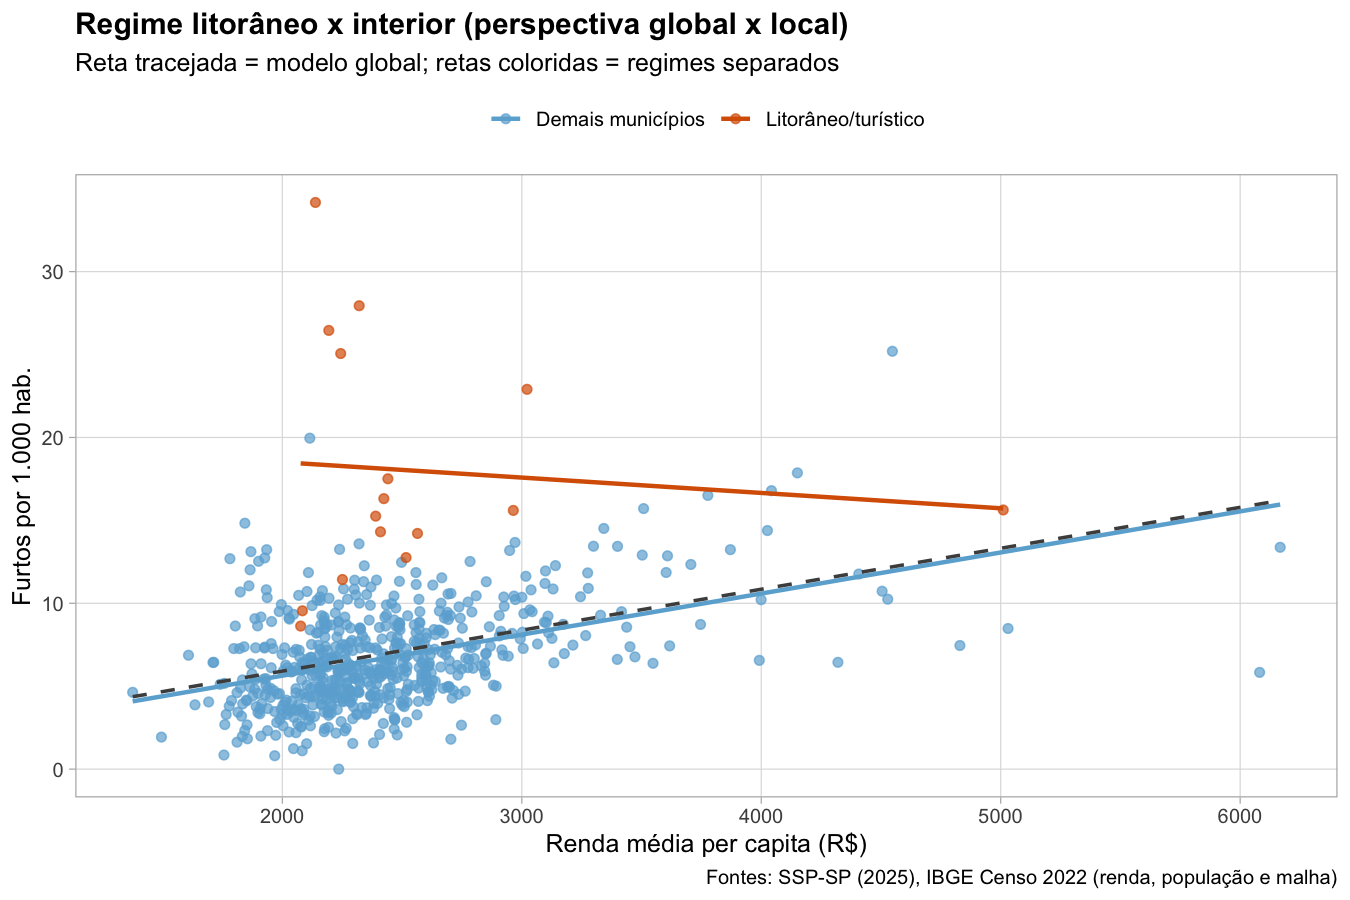
\includegraphics[width=0.9\linewidth]{litoral_regime_global_local.png}
\caption{Regressão por regime: litoral (laranja) contra interior (azul), e
modelo global (tracejado).}
\label{fig:regime}
\end{figure}

Por fim, o tratamento dos resíduos confirma o mecanismo (Fig.
\ref{fig:residuos}): sem a variável litoral, os municípios litorâneos têm
resíduo médio de $+10{,}68$ furtos/1.000 hab. contra $-0{,}27$ dos demais;
ao incluir a variável, os dois grupos centram em zero. A correlação entre o
resíduo (sem litoral) e a dummy litorânea é 0,51 e cai para 0,00 com a
variável incluída.

\begin{figure}[htbp]
\centering
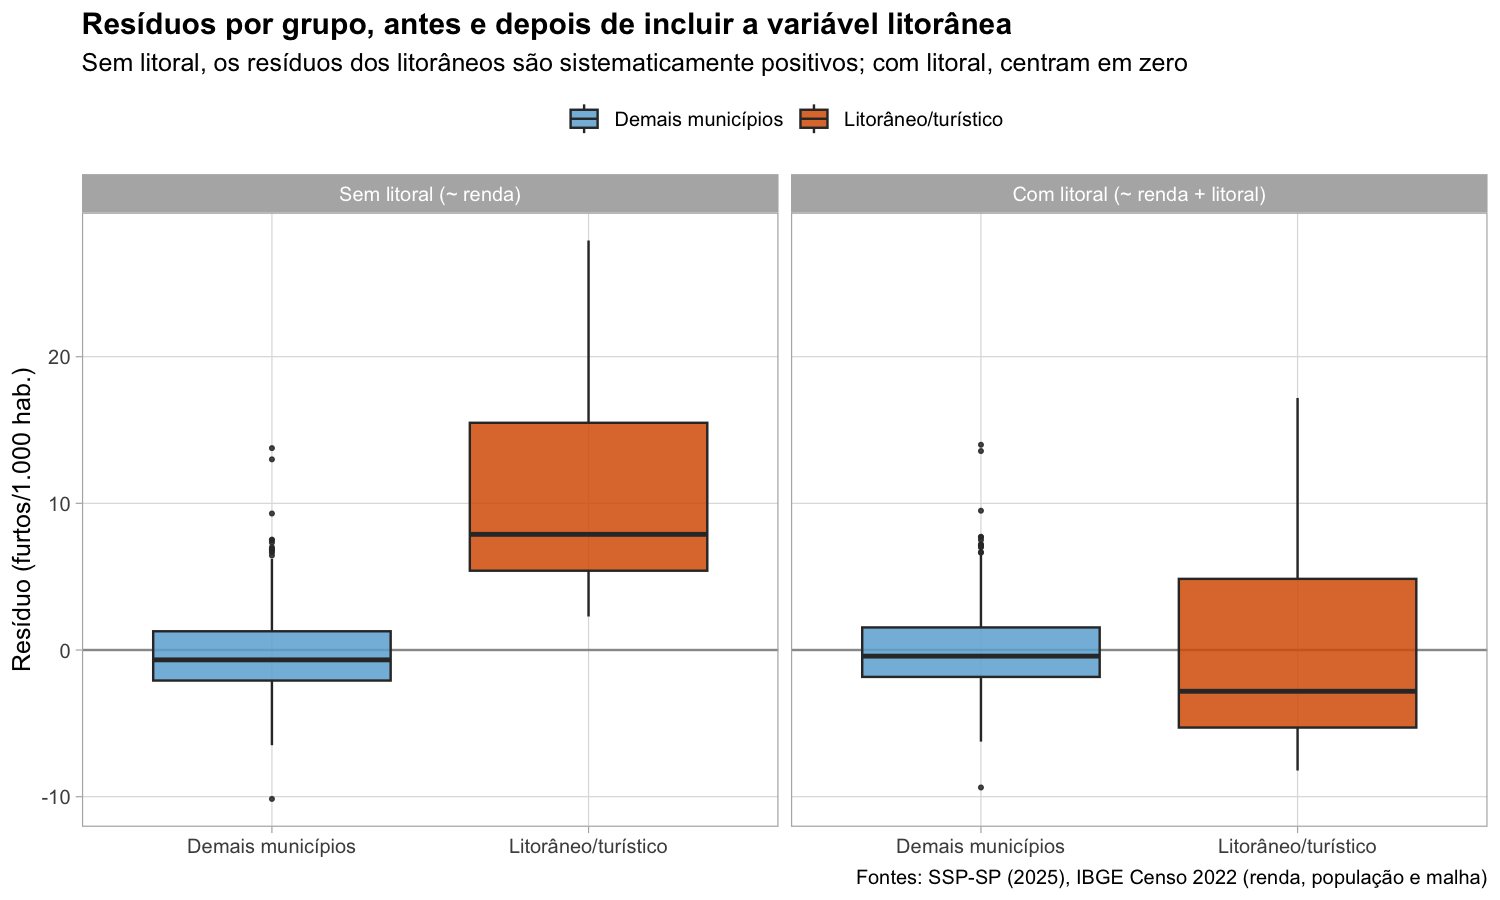
\includegraphics[width=0.9\linewidth]{residuos_litoral_boxplot.png}
\caption{Resíduos por grupo, com e sem a variável litorânea no modelo.}
\label{fig:residuos}
\end{figure}

\subsection{Comparação final dos modelos}

A Tabela \ref{tab:comparacao} compara os três tipos de modelo (OLS,
\textit{spatial error} e GWR) com e sem a variável litorânea, lado a lado,
para isolar o efeito de cada camada de complexidade. A condição litorânea
melhora o ajuste em todos os três casos, mas o ganho é desigual: é maior no
modelo mais simples ($\Delta R^2 = +0{,}228$ no OLS) e menor nos modelos
espaciais ($\Delta R^2 = +0{,}052$ no \textit{spatial error};
$+0{,}074$ no GWR) --- sinal de que os modelos espaciais já capturavam parte
do padrão litorâneo implicitamente, antes mesmo de a variável entrar
explicitamente. O melhor modelo entre todos os testados é o GWR com renda e
litoral, com $R^2 = 0{,}532$ e o menor AIC (3027,4).

\begin{table}[htbp]
\caption{Comparação de todos os modelos ajustados ($R^2$)}
\label{tab:comparacao}
\centering
\begin{tabular}{lccc}
\hline
\textbf{Modelo} & \textbf{Sem litoral} & \textbf{Com litoral} & $\boldsymbol{\Delta}$ \\
\hline
OLS & 0,129 & 0,357 & $+0{,}228$ \\
Spatial Error & 0,392 & 0,444 & $+0{,}052$ \\
GWR & 0,458 & \textbf{0,532} & $+0{,}074$ \\
\hline
\end{tabular}
\end{table}

\section{Conclusão}

A hipótese original deste trabalho --- de que municípios mais pobres
registram mais crimes patrimoniais --- não se sustenta nos dados de São
Paulo: a relação entre renda e taxa de furto é positiva, não negativa, tanto
na correlação simples quanto em todos os modelos de regressão testados. A
explicação mais consistente com a evidência acumulada é a hipótese
exploratória H2: municípios litorâneos e turísticos concentram taxas
elevadas de criminalidade patrimonial porque sua população flutuante de
verão infla o numerador da taxa sobre um denominador que mede apenas
residentes.

A progressão metodológica --- de correlação a Moran's I e LISA, de OLS a
\textit{spatial error} e finalmente a GWR --- revela três camadas distintas
do fenômeno: (i) a renda sozinha é insuficiente e deixa estrutura espacial
não explicada nos resíduos; (ii) essa estrutura é majoritariamente absorvida
por uma única variável omitida e espacialmente agrupada, a condição
litorânea; (iii) mesmo controlando por essa variável, a própria relação
renda--furto não é estacionária no espaço, sendo razoavelmente forte no
interior e quase nula no litoral, onde a dinâmica turística domina. O modelo
final (GWR com renda e litoral, $R^2 = 0{,}532$) combina essas duas camadas
e obtém o melhor ajuste entre todos os testados.

Como direção futura, a inclusão de uma medida direta de fluxo turístico
(hospedagem, pedágios, dados de telefonia) permitiria testar diretamente o
mecanismo proposto, hoje capturado apenas indiretamente por uma variável
dummy.

\section*{Agradecimentos}
Os autores agradecem à Prof.\textsuperscript{a} Flávia da Fonseca Feitosa
pela orientação ao longo da disciplina de Análise de Dados para
Planejamento Territorial.

\begin{thebibliography}{00}
\bibitem{moran1950} P. A. P. Moran, ``Notes on continuous stochastic
phenomena,'' \textit{Biometrika}, vol. 37, no. 1/2, pp. 17--23, 1950.
\bibitem{anselin1995} L. Anselin, ``Local indicators of spatial
association---LISA,'' \textit{Geographical Analysis}, vol. 27, no. 2,
pp. 93--115, 1995.
\bibitem{tobler1970} W. R. Tobler, ``A computer movie simulating urban
growth in the Detroit region,'' \textit{Economic Geography}, vol. 46,
sup. 1, pp. 234--240, 1970.
\bibitem{fotheringham2002} A. S. Fotheringham, C. Brunsdon, and M.
Charlton, \textit{Geographically Weighted Regression: The Analysis of
Spatially Varying Relationships}. Chichester: John Wiley \& Sons, 2002.
\bibitem{ibge} Instituto Brasileiro de Geografia e Estatística (IBGE),
\textit{Censo Demográfico 2022}. [Online]. Disponível em:
\url{https://censo2022.ibge.gov.br}
\bibitem{sspsp} Secretaria de Segurança Pública do Estado de São Paulo
(SSP-SP), \textit{Dados Estatísticos do Estado de São Paulo, 2025}.
[Online]. Disponível em: \url{https://www.ssp.sp.gov.br}
\end{thebibliography}

\end{document}
